% =====================================================================
%  SECTION 1 — INTRODUCTION ET CONTEXTE
% =====================================================================
\section{Introduction et Contexte}
\label{sec:intro}

\subsection{Cadre de la compétition BirdCLEF 2026}
La reconnaissance automatique d'espèces animales à partir de leur signature
acoustique constitue un enjeu majeur de la \textit{bioacoustique} contemporaine,
à la croisée de l'écologie quantitative, du traitement du signal et de
l'apprentissage statistique. Le projet s'inscrit dans le cadre de la
compétition Kaggle \textbf{BirdCLEF 2026}, dont l'aire d'étude est le
\textbf{Pantanal brésilien}, l'une des plus vastes zones humides de la
planète. La tâche consiste à prédire, pour chaque segment de \textbf{5~secondes}
d'environ 600 enregistrements de soundscapes de test, la probabilité
d'apparition de chacune des $K=234$ espèces du catalogue
(\textit{Aves}, \textit{Amphibia}, \textit{Mammalia}, \textit{Insecta},
\textit{Reptilia}).

\subsection{Problématique et formalisation}
Soit $\mathcal{D} = \{(s_i, \mathbf{y}_i)\}_{i=1}^{n}$ un ensemble de
$n$ segments audio $s_i \in \mathbb{R}^{T}$ échantillonnés à
$f_s = 32~\mathrm{kHz}$ ($T = 5 f_s = 160{,}000$ échantillons), associés à
un vecteur d'étiquettes binaires
$\mathbf{y}_i \in \{0,1\}^{K}$ encodant la présence simultanée des
espèces. La tâche n'est pas une classification multi-classe usuelle, mais un
problème de \textbf{classification multi-label}~: plusieurs espèces peuvent
coexister dans la même fenêtre temporelle. L'objectif est donc d'apprendre
une fonction
\[
    f_\theta : \mathbb{R}^{T} \longrightarrow [0,1]^{K},
    \qquad \hat{\mathbf{y}} = f_\theta(s),
\]
évaluée principalement à l'aide du \textbf{macro-ROC-AUC} et complétée par le
\textbf{macro F1-score} et la \textbf{mean Average Precision} (mAP), métriques
robustes au fort déséquilibre des classes.

\subsection{Hypothèses de travail}
Notre démarche repose sur quatre hypothèses, qui structurent l'ensemble du
pipeline de préparation des données~:
\begin{itemize}
    \item \textbf{H1 — Compacité spectrale.} L'information discriminante d'une
          vocalisation est largement contenue dans un vecteur compact de
          descripteurs temps-fréquence (MFCCs, contraste spectral, pitch, rythme), ce
          qui justifie une approche de type \textit{feature engineering} plutôt
          qu'un apprentissage \textit{end-to-end} sur le spectrogramme.
    \item \textbf{H2 — Séparabilité inter-taxa.} Les familles biologiques
          occupent des sous-bandes fréquentielles et des régimes rythmiques
          suffisamment distincts pour qu'un classifieur à base d'arbres puisse les
          séparer sans recourir à un réseau profond.
    \item \textbf{H3 — Prior géographique.} La distribution spatiale d'une
          espèce au sein du Pantanal apporte un \textit{biais inductif} non
          négligeable~: l'enrichissement par les coordonnées
          $(\text{lat}, \text{lon})$ doit améliorer la précision sans
          données acoustiques supplémentaires.
    \item \textbf{H4 — Décalage de domaine.} Les enregistrements focaux
          propres de \texttt{train\_audio/} et les soundscapes longs et bruités de
          \texttt{train\_soundscapes/} constituent deux distributions différentes ;
          cette dualité doit être traitée explicitement, sans quoi le modèle
          surapprend les signatures de microphone et non les espèces.
\end{itemize}

\subsection{Contributions et organisation du rapport}
Le présent rapport articule deux contributions complémentaires. Cette
première partie détaille la phase d'\textbf{analyse exploratoire} et de
\textbf{Data Engineering} : audit critique du corpus, conception d'un
pipeline DSP robuste, débruitage par traitement d'image, extraction
parcimonieuse de 158 descripteurs bioacoustiques, et enrichissement
spatial. La seconde partie, rédigée par notre binôme
(Section~\ref{sec:methode}), présente la \textbf{modélisation
    multi-label} et la comparaison expérimentale des classifieurs.
Les sections~\ref{sec:resultats} et~\ref{sec:critique} sont mutualisées.

% =====================================================================
%  SECTION 2 — ANALYSE DES DONNÉES
% =====================================================================
\section{Analyse des Données}
\label{sec:donnees}

\subsection{Présentation du corpus et écart de domaine}

\subsubsection{Sources hétérogènes}
Le corpus combine trois sous-ensembles structurellement différents,
résumés dans la Table~\ref{tab:corpus}. Cette hétérogénéité, loin d'être
un détail, conditionne la stratégie de validation et d'augmentation~:
les enregistrements focaux issus de \textit{xeno-canto} et
\textit{iNaturalist} sont propres, courts et centrés sur un individu, alors
que les soundscapes captent un \textbf{paysage sonore} complet, avec
recouvrement d'espèces, bruit de pluie, vent et insectes nocturnes.

\begin{table}[h]
    \centering
    \small
    \begin{tabular}{lccc}
        \hline
        \textbf{Source}              & \textbf{Durée typique} & \textbf{Densité d'espèces} &
        \textbf{Bruit de fond}                                                                      \\
        \hline
        \texttt{train\_audio/}       & 5--40~s                & 1 (+ secondaires)          & faible \\
        \texttt{train\_soundscapes/} & 60~s                   & multiples                  & élevé  \\
        \texttt{test\_soundscapes/}  & 60~s                   & multiples (caché)          & élevé  \\
        \hline
    \end{tabular}
    \caption{Caractéristiques des trois sous-ensembles du corpus BirdCLEF~2026.}
    \label{tab:corpus}
\end{table}

\paragraph{Critique.} Cette dissymétrie engendre un \textbf{covariate shift}
dont l'effet est largement sous-estimé dans la littérature appliquée~: un
modèle entraîné majoritairement sur les focaux apprend à reconnaître des
chants \textit{en isolation}, mais sera évalué sur des chants
\textit{mélangés}. C'est l'une des principales sources d'erreurs anticipées
(cf.~Section~\ref{sec:critique}).

\subsubsection{Analyse qualitative des enregistrements}
La métadonnée \texttt{rating} ($\in [0;5]$) attribuée par les contributeurs
de \textit{xeno-canto} fournit un indice de qualité subjectif. La
Figure~\ref{fig:rating} en révèle une distribution \textbf{fortement
    bimodale}~: un pic massif à $0$ (qualité non renseignée, $\approx 13{,}000$
enregistrements) et un mode dominant entre $4$ et $5$. La médiane sur les
valeurs renseignées s'établit à $3{,}5$.

\begin{figure}[h]
    \centering
    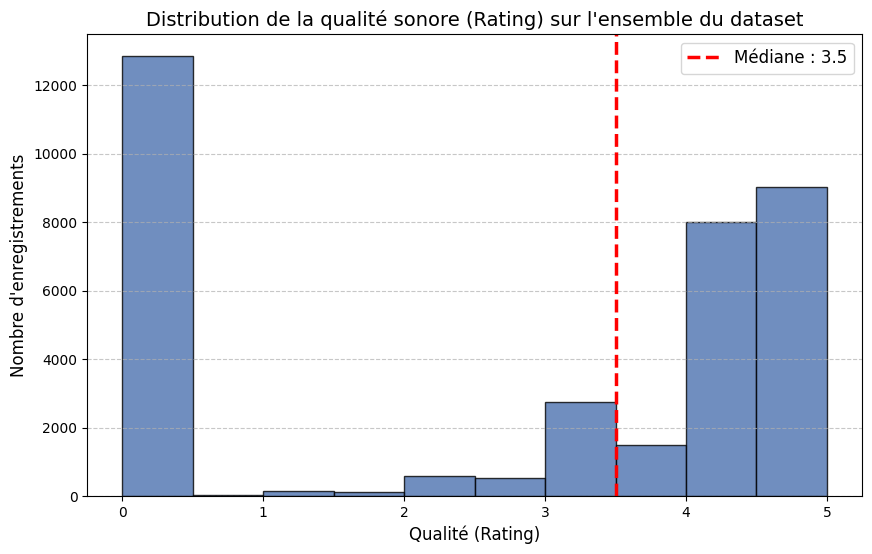
\includegraphics[width=0.78\linewidth]{Plot/distribution_qualité.png}
    \caption{Distribution du \texttt{rating} sur l'ensemble du corpus
        \texttt{train\_audio/}. La valeur $0$ (non renseignée) concentre près
        d'un tiers des enregistrements et a été exclue des statistiques
        qualitatives globales.}
    \label{fig:rating}
\end{figure}

\paragraph{Choix méthodologique.} Plutôt que d'exclure les fichiers de
faible \texttt{rating}, qui auraient amputé le corpus de classes déjà
sous-représentées, nous avons~: (i) \textbf{requalifié} \texttt{rating}$=0$
comme « inconnu » et non « mauvais » ; (ii) \textbf{conservé} l'ensemble du
corpus pour préserver la couverture taxonomique~; (iii) reporté la
robustesse au bruit sur la chaîne DSP. Ce choix est délibérément
conservateur~: la perte d'information taxonomique nous a paru plus
dommageable qu'un léger bruit d'apprentissage.

\subsubsection{Déséquilibre de classes et difficulté multi-label}
Le catalogue de $K=234$ classes est intrinsèquement déséquilibré~: certaines
espèces sont représentées par plusieurs centaines de fichiers,
d'autres (notamment certains \textit{sonotypes} d'insectes du type
\texttt{47158son16}, dont l'espèce exacte n'est pas identifiée par les
experts) ne le sont que par une poignée d'occurrences. De surcroît,
\textit{certaines espèces n'apparaissent que dans les soundscapes et jamais
    dans les focaux}, ce qui rend impossible une simple stratégie
d'entraînement sur \texttt{train\_audio/} seul.

\subsection{Caractérisation temps-fréquence des familles}

\subsubsection{Lecture comparée des spectrogrammes}
La Figure~\ref{fig:specs} compare des Mel-spectrogrammes nettoyés
représentatifs des cinq familles. La lecture est éclairante~:
\textit{Reptilia} (cf.~Figure~\ref{fig:specs}, en bas) présente
des cris transitoires courts, larges en bande, accompagnés
de stridulations d'insectes continues vers $8$~kHz~;
\textit{Amphibia} (cf.~Figure~\ref{fig:specs}, milieu) montre une
bande étroite quasi-permanente autour de $2{,}5$~kHz superposée à
des cris brefs basse fréquence~; les \textit{Aves} concentrent leur
énergie entre $2$ et $8$~kHz, en motifs syllabiques structurés.

\begin{figure}[h]
    \centering
    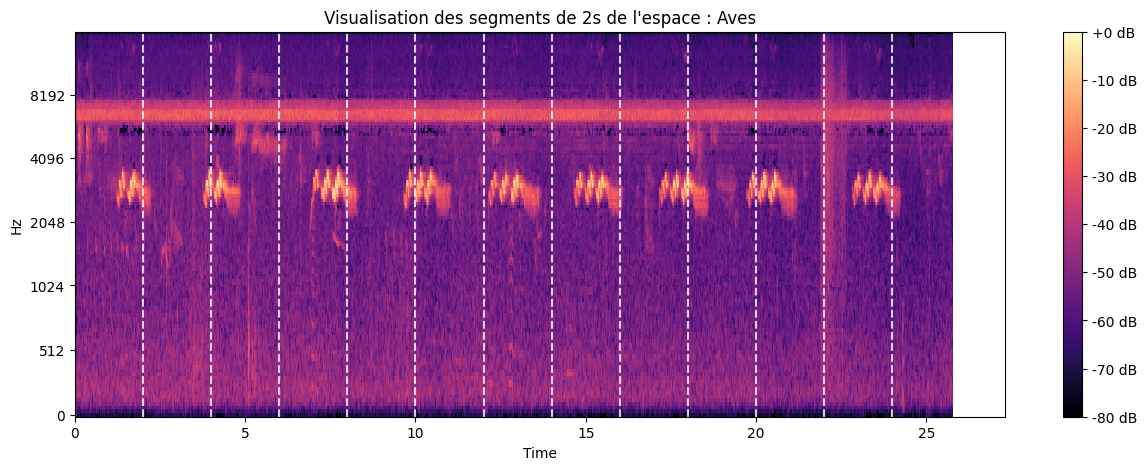
\includegraphics[width=0.95\linewidth]{Plot/MELOSPLI.png}\\[2pt]
    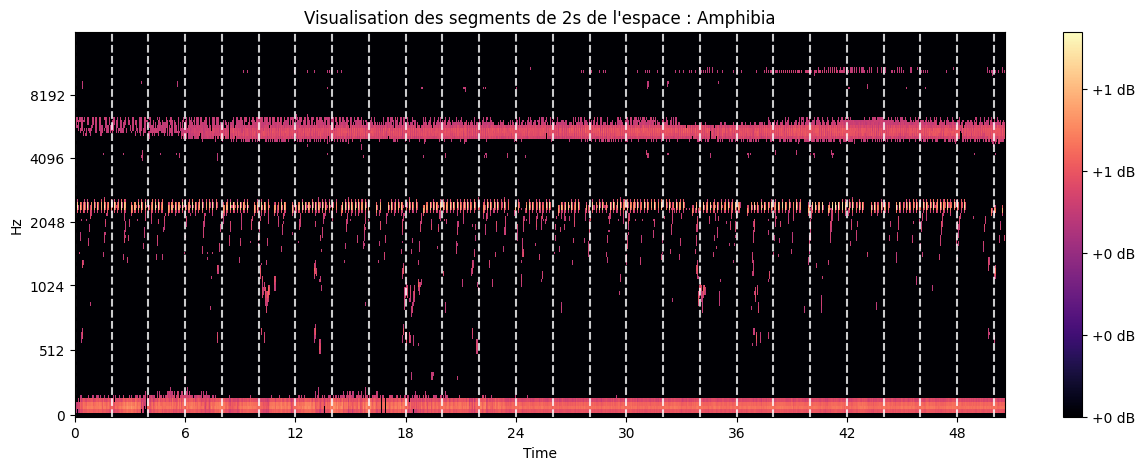
\includegraphics[width=0.95\linewidth]{Plot/MELOSPLOTCLEAN.png}\\[2pt]
    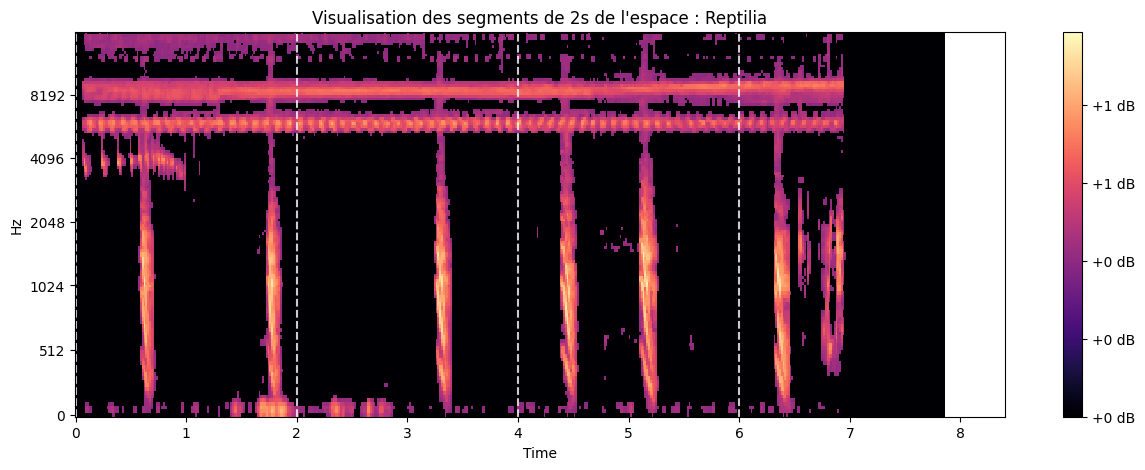
\includegraphics[width=0.95\linewidth]{Plot/MELOSPLITCLEAN2.png}
    \caption{Mel-spectrogrammes nettoyés (algorithme « Karcher ») pour les
        familles \textit{Aves}, \textit{Amphibia} et \textit{Reptilia}. Les
        pointillés blancs marquent les frontières des segments de 2~s utilisées
        en analyse exploratoire ; le pipeline final segmente à 5~s.}
    \label{fig:specs}
\end{figure}

\paragraph{Implication pour le feature engineering.} Ces observations
visuelles motivent directement le choix de descripteurs qui agrègent
l'énergie sur des \textbf{sous-bandes fréquentielles} (8 bandes du
Mel-spectrogramme débruité, plage active min/max/largeur) et qui
quantifient la \textbf{structuration temporelle} (rythme syllabique,
proportion de \textit{frames} actives).

\subsubsection{Indice de Coïncidence comme descripteur de pureté locale}
Inspiré de la cryptanalyse classique, nous proposons d'appliquer un
\textbf{Indice de Coïncidence} (IC) sur les distributions d'amplitude
quantifiées de chaque sous-segment de ${,}5$~s. L'IC d'une distribution
discrète $(p_1, \dots, p_M)$ s'écrit
\[
    \mathrm{IC} = \sum_{k=1}^{M} p_k\,(p_k - 1) \cdot \frac{1}{N(N-1)} \cdot N^2,
\]
et mesure la « pureté locale »~: une distribution concentrée
(son tonal pur) donne une valeur élevée, une distribution uniforme
(bruit blanc) tend vers $1$. Les figures~\ref{fig:ic_moy}
et~\ref{fig:ic_ind} démontrent un \textbf{pouvoir séparateur tangible} entre
\textit{Insecta} (IC moyen $\approx 9$--$11$, stridulation très tonale et
stable) et \textit{Aves}/\textit{Mammalia} (IC $\approx 3$--$4$, signal plus
diffus). Les profils individuels confirment qu'au-delà de la moyenne, c'est
la \textbf{dynamique temporelle} de l'IC qui discrimine les familles.

\begin{figure}[h]
    \centering
    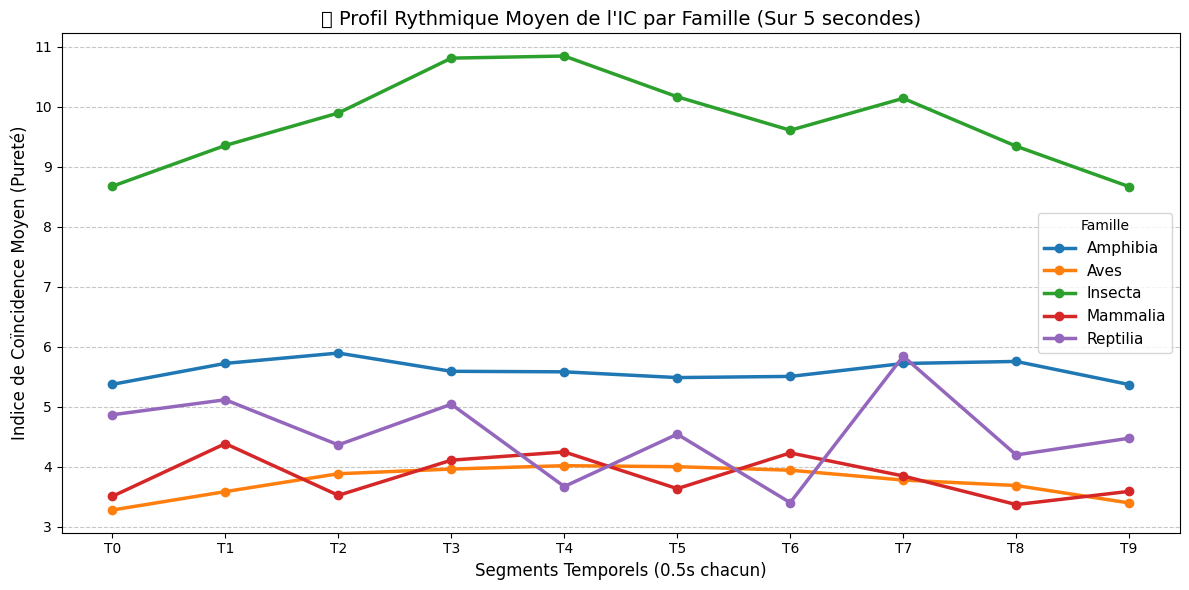
\includegraphics[width=0.85\linewidth]{Plot/IC.png}
    \caption{Profil rythmique moyen de l'Indice de Coïncidence par famille
        biologique, calculé sur 10 sous-segments de 0,5~s. Les \textit{Insecta}
        se détachent nettement.}
    \label{fig:ic_moy}
\end{figure}

\begin{figure}[h]
    \centering
    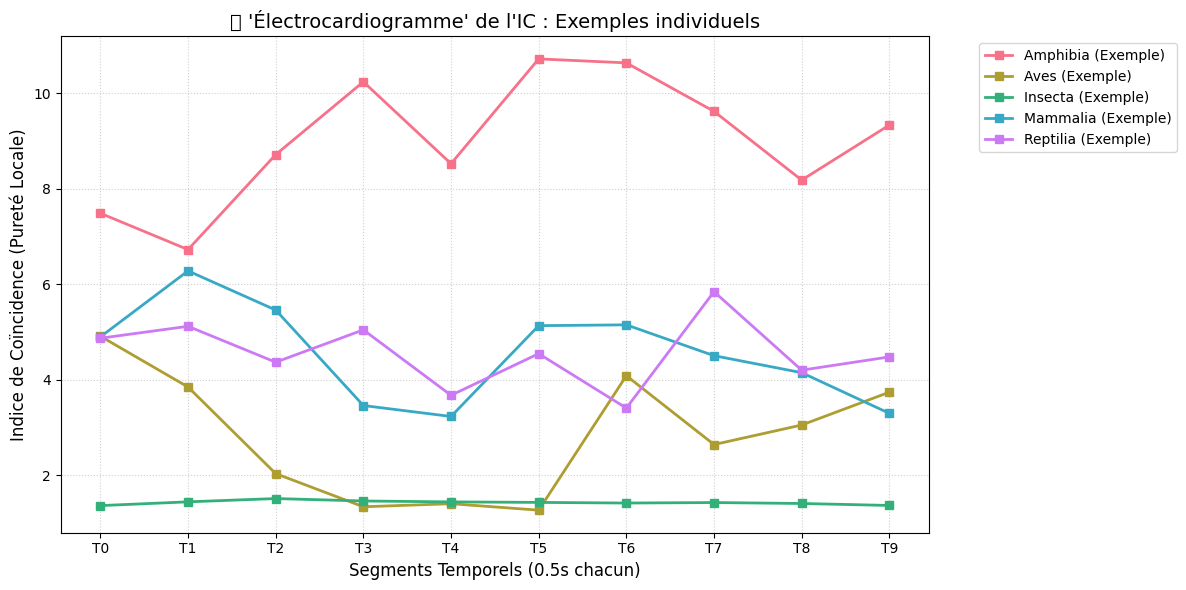
\includegraphics[width=0.85\linewidth]{Plot/IC2.png}
    \caption{Trajectoires individuelles d'IC : la dynamique temporelle
        (variance, périodicité) est elle-même un descripteur.}
    \label{fig:ic_ind}
\end{figure}

\subsection{Pipeline de préparation et de nettoyage}

\subsubsection{Conditionnement du signal (DSP)}
Chaque clip subit un prétraitement strict avant toute extraction~:
\begin{itemize}
    \item \textbf{Standardisation} à $f_s = 32~\mathrm{kHz}$.
    \item \textbf{DC offset removal}~: $s \leftarrow s - \overline{s}$, qui
          stabilise les estimations d'énergie et de pitch.
    \item \textbf{Troncation} des 500 premiers échantillons pour supprimer
          les transitoires d'amorçage du microphone.
    \item \textbf{Fade-in / fade-out} linéaire de 50~ms aux extrémités pour
          annuler les clics aux frontières de découpe.
    \item \textbf{Pré-emphase} via filtre passe-haut, compensant
          l'atténuation naturelle des hautes fréquences (cruciale pour les
          sifflements de passereaux).
    \item \textbf{Fenêtrage de Hanning} avant FFT, pour limiter le
          \textit{spectral leakage}.
\end{itemize}

\paragraph{Localisation du segment utile.} Pour chaque clip focal long,
nous extrayons par \textbf{fenêtrage RMS glissant} (fenêtre 5~s, pas 0,5~s)
le segment maximisant
\[
    E_{\mathrm{RMS}}(t) = \sqrt{\frac{1}{W}\sum_{k=t}^{t+W-1} s[k]^2}.
\]
Cette stratégie évite d'entraîner le modèle sur des secondes de silence ou
de respiration parasitaire (Figure~\ref{fig:energie}).

\begin{figure}[h]
    \centering
    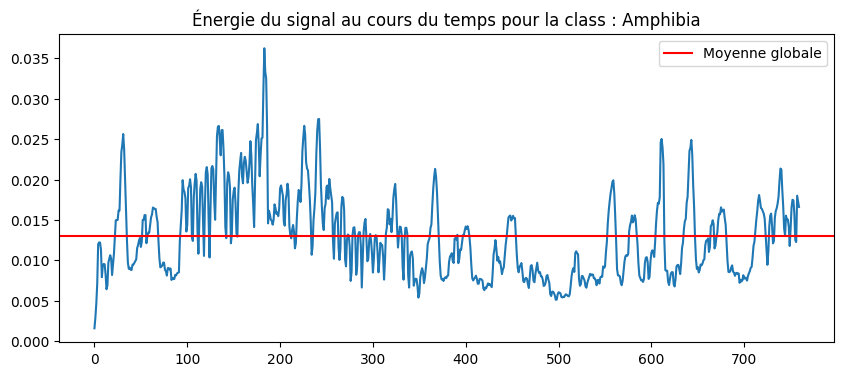
\includegraphics[width=0.8\linewidth]{Plot/ANALYSENERGIE.png}
    \caption{Énergie temporelle d'un enregistrement \textit{Amphibia}.
        La forte variance valide l'usage d'un fenêtrage RMS pour cibler la
        portion biologiquement informative.}
    \label{fig:energie}
\end{figure}

\subsubsection{Débruitage « Karcher » par traitement d'image 2D}
Le bruit de fond du Pantanal (pluie, insectes nocturnes, vent dans la
canopée) est \textit{stationnaire à large bande}~: les techniques
classiques de \textit{spectral subtraction} y sont peu efficaces.
Nous traitons donc le Mel-spectrogramme $S \in \mathbb{R}^{F \times T}$
comme une image et lui appliquons trois opérations successives~:
\begin{enumerate}
    \item \textbf{Normalisation Min-Max} sur $[0,1]$ pour homogénéiser
          l'échelle des bandes ;
    \item \textbf{Filtrage médian 2D} (\texttt{skimage}, élément structurant
          \texttt{disk(1)}), qui élimine le bruit poivre-et-sel sans flouter les
          fronts d'attaque ;
    \item \textbf{Seuillage dynamique} $S \leftarrow S \cdot \mathds{1}_{S
                  > 1{,}5 \cdot \mathrm{median}(S)}$, isolant les pics d'énergie réels.
\end{enumerate}

\paragraph{Analyse critique du débruitage.} L'algorithme est volontairement
agressif. Son intérêt est démontré sur les statistiques d'énergie par
sous-bande (Section~\ref{sec:features}), mais il introduit un risque
identifié~: les vocalisations \textbf{distantes et faibles} (espèces
rares, individus en arrière-plan) peuvent être annihilées par le seuillage.
Nous mitigons partiellement ce biais en conservant en parallèle des
descripteurs calculés sur le \textbf{spectrogramme non nettoyé} (MFCCs,
centroïde, contraste, flatness), garantissant que l'information de bas
niveau ne soit pas perdue. Cette redondance contrôlée est, à notre sens,
préférable à un seuillage adaptatif plus sophistiqué qui aurait alourdi
le pipeline sans garantie de gain.

\subsection{Extraction de 158 caractéristiques bioacoustiques}
\label{sec:features}

\subsubsection{Vue d'ensemble du vecteur de descripteurs}
Chaque segment de 5~s est compressé en un vecteur
$\mathbf{x}_i \in \mathbb{R}^{d}$ avec $d=158$ descripteurs acoustiques,
porté ensuite à $d=160$ par l'enrichissement spatial. La
Table~\ref{tab:features} récapitule la composition.

\begin{table}[h]
    \centering
    \small
    \begin{tabular}{lcl}
        \hline
        \textbf{Famille de descripteurs}           & \textbf{Dim.} & \textbf{Rôle biologique principal} \\
        \hline
        MFCCs (20 coeff. $\times$ 4 stats)         & 80            & timbre vocal                       \\
        Delta-MFCCs (13 $\times$ 2)                & 26            & dynamique transitoire              \\
        Spectral centroid                          & 2             & hauteur globale                    \\
        Spectral contrast (7 bandes)               & 14            & harmonicité                        \\
        Spectral flatness                          & 2             & tonalité vs bruit                  \\
        Zero-Crossing Rate                         & 2             & percussivité                       \\
        Fréquence fondamentale $F_0$               & 4             & hauteur tonale                     \\
        Modulation de fréquence                    & 3             & trilles, glissandos                \\
        Mel-spectro débruité (8 bandes)            & 16            & cartographie spectrale             \\
        Frames actives                             & 1             & densité d'événements               \\
        Syllabes et rythme                         & 5             & cadence d'émission                 \\
        Plage fréquentielle active                 & 3             & filtre biologique                  \\
        \hline
        \textbf{Total acoustique}                  & \textbf{158}  &                                    \\
        $+$ Latitude / Longitude (bonus non-audio) & $+2$          & \textit{prior} géographique        \\
        \hline
        \textbf{Total final $d$}                   & \textbf{160}  &                                    \\
        \hline
    \end{tabular}
    \caption{Composition du vecteur de caractéristiques $\mathbf{x}_i$.}
    \label{tab:features}
\end{table}

\paragraph{Justification du \textit{feature engineering} face à
    l'\textit{end-to-end}.} L'approche par descripteurs experts s'oppose
ici aux architectures de type AST ou Swin Transformer, qui dominent
l'état de l'art (cf. Section~\ref{sec:methode}). Notre choix est
\textit{contraint} et \textit{assumé}~: la compétition impose une
inférence CPU plafonnée à 90~min pour 600 fichiers, ce qui rend
prohibitif un Transformer fenêtré pleine résolution. Un vecteur
$\mathbb{R}^{160}$ injecté dans un ensemble d'arbres offre un compromis
favorable entre \textit{capacité de modélisation} et \textit{débit
    d'inférence}, tout en restant interprétable~— condition essentielle pour
diagnostiquer les cas d'erreur.

\subsubsection{Sélection statistique : ANOVA F-test}
La pertinence individuelle des descripteurs a été évaluée par une
\textbf{ANOVA unidirectionnelle} (\texttt{scipy.stats.f\_oneway}).
Pour un descripteur $x^{(j)}$ et $K$ classes,
\[
    F^{(j)} = \frac{\mathrm{Var}_{\text{inter}}(x^{(j)})}
    {\mathrm{Var}_{\text{intra}}(x^{(j)})}.
\]
Les scores ont confirmé la supériorité \textit{statistiquement
    significative} des descripteurs d'ordre supérieur~: \textit{kurtosis} et
\textit{skewness} spectrales, \textit{entropie de Shannon},
\textbf{Acoustic Complexity Index} (ACI) et énergie PCEN dépassent
nettement les MFCCs basiques pris individuellement. Cette analyse a guidé
la décision de conserver MFCCs + Deltas comme socle bas niveau, mais d'y
adjoindre systématiquement les descripteurs d'ordre 2 et 3.

\subsubsection{Estimateur de pitch sur-mesure (note d'ingénierie)}
L'extraction de la fréquence fondamentale $F_0$ par
\texttt{librosa.yin} provoquait des \textit{segmentation faults}
systématiques sur architecture Apple Silicon, dus à l'incompatibilité de
Numba JIT en multiprocessus fork. Nous avons réimplémenté un estimateur
par \textbf{autocorrélation pure NumPy} dans
\texttt{DataProcessing.py}, recherchant le pic d'autocorrélation dans
la bande $[200~\mathrm{Hz},\,10~\mathrm{kHz}]$ adaptée à la bioacoustique.
Cette implémentation est stable (zéro crash sur les 10~658
soundscapes traités) et conserve la dimensionnalité exacte des features,
préservant la compatibilité descendante du pipeline.

\subsection{Bonus 1 — Exploitation de données non-audio}
\label{sec:bonus_geo}

Au-delà du signal acoustique, nous injectons explicitement les
\textbf{coordonnées géographiques} $(\text{lat}, \text{lon})$ comme
features d'entrée du classifieur. Pour les enregistrements focaux, ces
coordonnées proviennent de la colonne dédiée de \texttt{train.csv}~; pour
les soundscapes du Pantanal, dépourvus de coordonnées individuelles, nous
attribuons les coordonnées centroïdes de la zone d'étude
$(-19{,}05,\;-56{,}75)$.

\paragraph{Pourquoi cela compte.} La distribution d'une espèce est par
nature géo-conditionnée~: deux espèces produisant des cris acoustiquement
voisins peuvent être facilement disambiguées si l'une n'est observée
qu'au nord de la zone et l'autre qu'au sud. Un arbre de décision
LightGBM peut exploiter directement ces deux dimensions pour
\textbf{couper l'espace de prédiction} en zones biologiquement
plausibles, sans modèle géographique explicite. Cet enrichissement,
quasi-gratuit, constitue l'un de nos bonus revendiqués.

\subsection{Bonus 2 — Descripteurs visuels et signatures de famille}

En traitant le Mel-spectrogramme nettoyé comme une image 2D, nous avons
exploré trois familles de descripteurs issus de la vision par ordinateur~:
\begin{itemize}
    \item \textbf{SIFT} (\texttt{cv2.SIFT\_create}) sur le spectrogramme
          converti en \texttt{uint8}~: extraction des 10 \textit{keypoints} les
          plus énergétiques, agrégés en un vecteur fixe de 1280 dimensions.
    \item \textbf{Détection de \textit{blobs}} par Laplacien de Gaussienne
          (\texttt{skimage.feature.blob\_log}) pour compter les évènements
          acoustiques denses (Figure~\ref{fig:blobs}).
    \item \textbf{Histogrammes de gradients orientés} (HOG) pour modéliser
          les contours géométriques des syllabes.
\end{itemize}

\begin{figure}[h]
    \centering
    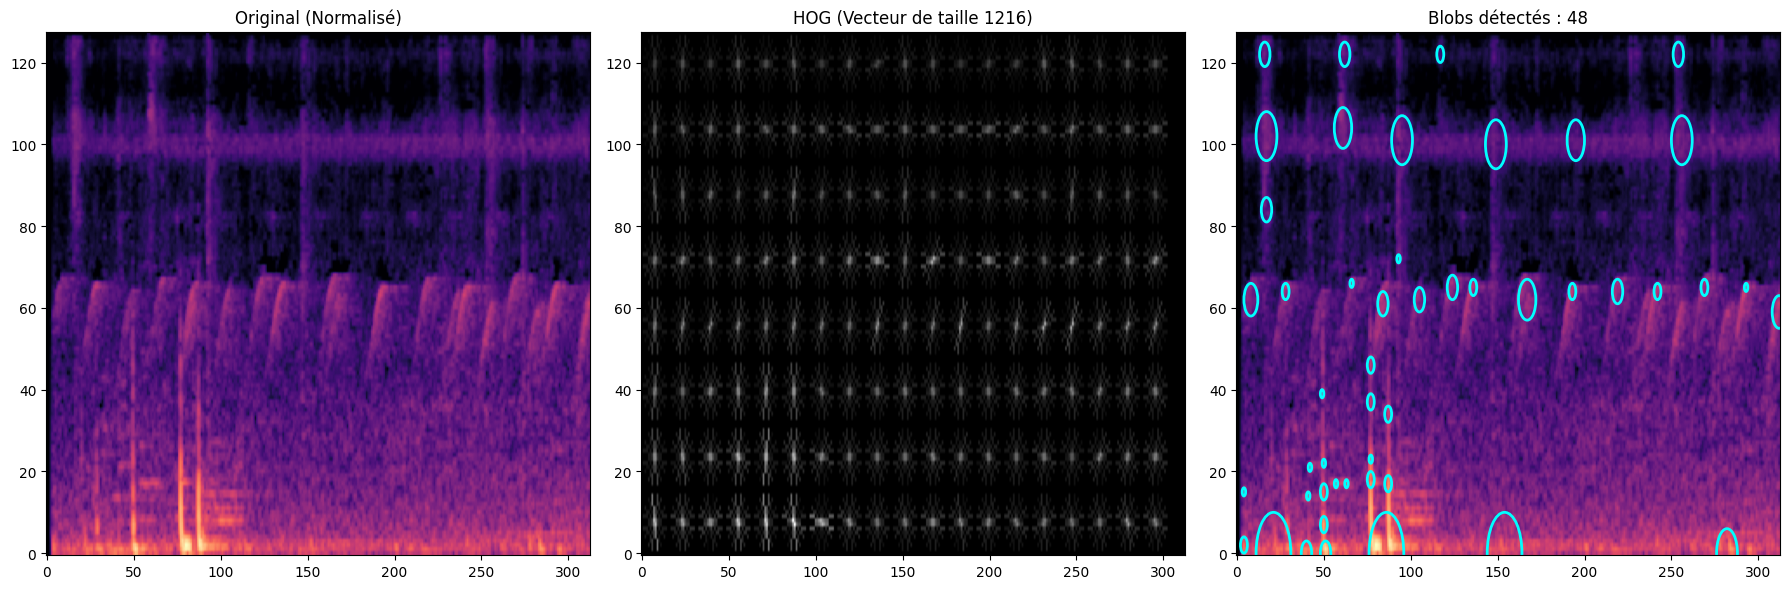
\includegraphics[width=0.9\linewidth]{Plot/BLOBIMAGERIE.png}
    \caption{Pipeline d'analyse visuelle d'un spectrogramme~: original
        normalisé (gauche), HOG (centre), blobs détectés par
        LoG (droite, 48 blobs).}
    \label{fig:blobs}
\end{figure}

Par projection \textbf{t-SNE} des signatures SIFT moyennes
(Figure~\ref{fig:tsne}), nous constatons que l'espace latent acoustique
forme une variété continue plutôt que des clusters nets par famille~: ce
résultat, négatif en apparence, est diagnostique~— il montre que les
descripteurs visuels seuls ne suffisent pas à séparer les taxa, et
justifie a posteriori notre choix de les combiner aux descripteurs DSP.

\begin{figure}[h]
    \centering
    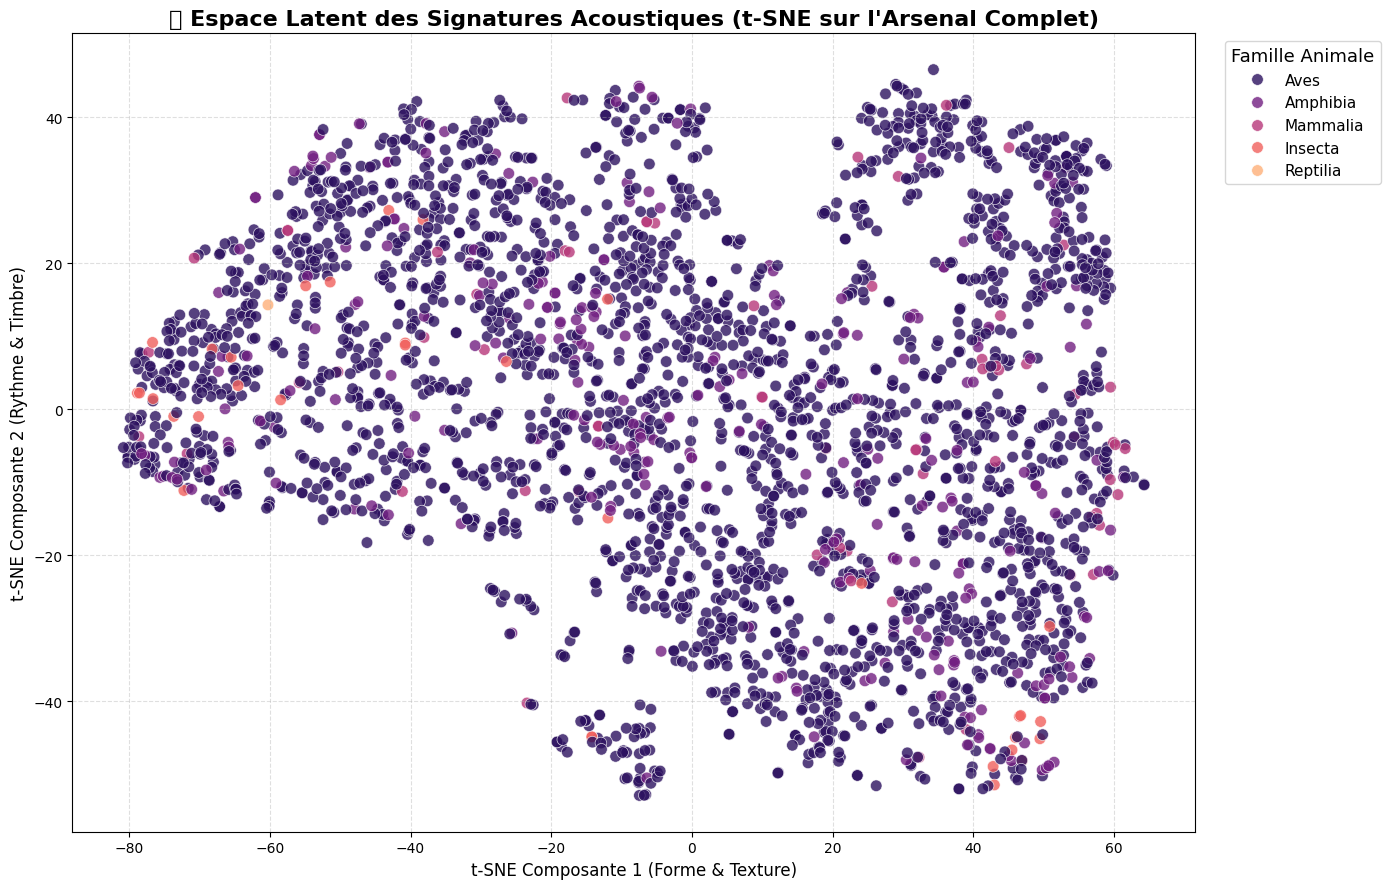
\includegraphics[width=0.7\linewidth]{Plot/tsne-IC.png}
    \caption{Projection t-SNE des signatures acoustiques (forme et texture).
        L'absence de cluster franc par famille animale révèle un fort
        recouvrement inter-taxa dans l'espace des descripteurs visuels,
        motivant l'usage complémentaire des descripteurs DSP.}
    \label{fig:tsne}
\end{figure}

\subsection{Stratégie de traitement à l'échelle et prévention du
    \textit{data leakage}}

\subsubsection{Industrialisation du calcul}
L'extraction sur l'intégralité du corpus
($\sim 10{,}658$ soundscapes $+$ enregistrements focaux) impose une
contrainte d'ingénierie sérieuse. Nous avons~:
\begin{itemize}
    \item forcé les spectrogrammes Mel en \texttt{float32}
          ($-50\%$ de RAM)~;
    \item segmenté l'extraction en \textit{mini-batches} de 50 fichiers
          pour stabiliser le \textit{garbage collector}~;
    \item parallélisé via \texttt{joblib.Parallel} avec backend
          \texttt{loky}~;
    \item persisté les vecteurs au format \textbf{Apache Parquet}
          (typage strict, lecture colonne)~;
    \item ajouté une sauvegarde progressive \texttt{try/except/finally}
          permettant de reprendre un traitement interrompu sans perte.
\end{itemize}

\subsubsection{Prévention rigoureuse du \textit{data leakage}}
Deux pièges classiques ont été identifiés et neutralisés~:
\begin{itemize}
    \item \textbf{Scaling sans fuite.} Le \texttt{StandardScaler} est
          calibré uniquement sur l'ensemble d'entraînement
          (\texttt{fit\_transform}) puis appliqué de façon passive
          (\texttt{transform}) sur la validation.
    \item \textbf{Fuite par fichier source.} Un même clip de 60~s génère
          12 segments de 5~s très corrélés. Un \texttt{train\_test\_split}
          naïf placerait certains segments d'un même fichier dans le train et
          d'autres dans la validation, ce qui surestimerait massivement les
          performances. La stratégie correcte, \textbf{StratifiedGroupKFold}
          groupé par \texttt{filename}, est explicitée dans la
          Section~\ref{sec:methode} de notre binôme.
\end{itemize}

\subsection{Transition vers la méthode proposée}
\label{sec:transition}

À l'issue de cette phase, le corpus brut a été transformé en une matrice
de descripteurs
\[
    \mathbf{X} \in \mathbb{R}^{n \times d},
    \qquad
    \mathbf{Y} \in \{0,1\}^{n \times K},
    \qquad
    d = 160,\; K = 234,
\]
strictement standardisée, persistée en Parquet, et alignée entre focaux
et soundscapes. La structure même de $\mathbf{Y}$
(multi-label, fortement déséquilibrée, à classes partiellement absentes en
validation) appelle un \textit{wrapper} adapté autour d'un classifieur de
base. La Section~\ref{sec:methode} détaille ce choix~: nous comparons un
\textbf{LightGBM} encapsulé dans un \texttt{MultiOutputClassifier} à une
baseline plus simple, et discutons l'opportunité d'une comparaison
ultérieure à des \textbf{embeddings pré-entraînés} (Google Perch,
BirdNET) que les Transformers récents (AST, Swin) ont popularisés mais
qui restent contraints par le budget CPU imposé par Kaggle.